\documentclass{article}

\usepackage[pdftex]{graphicx}
\usepackage{amsmath}
\usepackage{amssymb}
\usepackage{hyperref}
\usepackage{tkz-orm}
\usepackage[utf8]{inputenc}
\usepackage{graphicx}
\usepackage[english,dutch]{babel}
\usepackage{caption}
\usepackage{subcaption}
\usepackage[section]{placeins}

\author{Thom Wiggers\\ s4119444}
\title{Informatiesystemen 1}

\newcommand{\Spec}{\ensuremath{\operatorname{Spec}}}
\newcommand{\Gen}{\ensuremath{\operatorname{Gen}}}
\newcommand{\Base}{\ensuremath{\operatorname{Base}}}
\newcommand{\total}{\ensuremath{\operatorname{total}}}

\begin{document}
\maketitle
\tableofcontents
\section{Huishoudelijke mededelingen}
Dit project maak ik individueel. 

\section{Taak 1 - ORC vs. SQL}
\subsection{Inleiding}
ORM is een methode om door middel van modellen systemen te ontwikkelen waarbij
gepoogd wordt zo min mogelijk fouten toe te laten en zo veel mogelijk
redundantie in de opgeslagen gegevens te voorkomen. 

ORM bestaat voornamelijk uit een verzameling afspraken over taalgebruik en
notaties. Hierdoor zou een goed model ook voor niet-domeinexperts leesbaar
en begrijpbaar moeten zijn. 

Hoewel ORM modellen vooral worden omgezet naar klassieke relationele
(SQL)-databases, is het ook mogelijk om direct 'vragen` te stellen aan
een dataset in ORM. Deze querytaal staat bekend als Object-Role Calculus 
(ORC).

Ik ga hier proberen ORC te vergelijken met de SQL taal, door middel van het
vergelijken van enkele verschillende queries, zoekvragen, waarbij ik ook 
in ga op de fundamentele verschillen tussen de twee verschillende systemen.
Hiervoor zal ik een voorbeeldsysteem beschrijven, zowel uitgevoerd in ORM 
als draaiende op de populaire relationele database postgreSQL.

\subsection{Systeem}
Ik ga hier een voorbeeldsysteem beschrijven van een webwinkel waar men 
schoenen verkoopt. In deze webwinkel houdt men bestellingen bij, en 
profielen van klanten. Bestellingen kunnen bestaan uit een of meerdere
paren schoenen, in verschillende maten en aantallen.

\subsubsection{ORM}
\begin{figure}[htp]
  \centering
  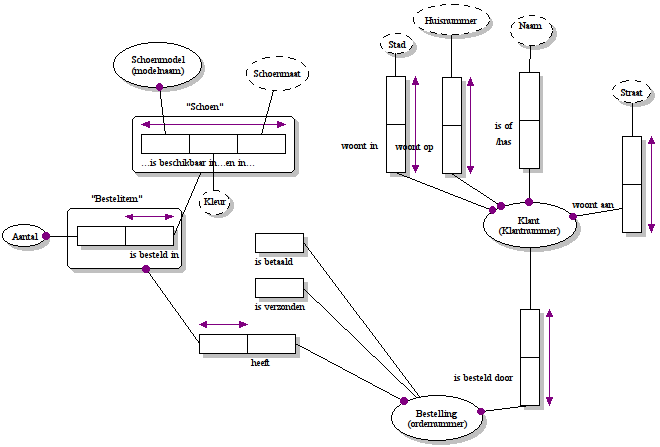
\includegraphics[keepaspectratio=true, width=345pt]{model1.png}
  \caption{ORM Model van het voorbeeldsysteem}
  \label{img:model1}
\end{figure}

\Large{--- Check syntax --- }
\Large{Todo: Fix diagram: Naam, constraint Schoen}

\begin{verbatim}
Schoen: Schoenmodel (modelnaam) is beschikbaar
    in Schoenmaat en is beschikbaar in Kleur.
Bestelitem: Schoen is besteld in aantal.
Bestelling (ordernummer) heeft Bestelitem.
Bestelling (ordernummer) is besteld door 
   Klant (klantnummer).
Bestelling is betaald.
Bestelling is verzonden.
Klant (klantnummer) woont aan 
   Straat (straatnaam).
Klant (klantnummer) woont op 
   Huisnummer (nr).
Klant (klantnummer) woont in Stad (naam).
Klant (klantnummer) heet Naam.
\end{verbatim}

\subsubsection{SQL Tabellen}

Het transformeren van het ORM model naar SQL tabellen is redelijk 
eenvoudig, maar om dubbel voorkomende gegevens te voorkomen heb ik
op verschillende plaatsen een identificatienummer aan tabellen 
toegevoegd als vervangende primary key.

Hier wordt al een duidelijk nadeel van SQL-gebaseerde databases
zichtbaar: het is niet mogelijk om gegevens te objectiviseren.

Zie hiervoor de tabellen \ref{tab:schoen}, \ref{tab:bestelitem},
\ref{tab:bestellingen}, \ref{tab:bestelitembestelling} en \ref{tab:klant}.

\begin{table}[hp]
  \centering
  \begin{tabular}{l|l|l|l}
    \textbf{id} & \textbf{Schoenmodel} & \textbf{Kleur} & \textbf{Schoenmaat} \\
    \hline
    1 & Model a              & Zwart          & 43 \\
    2 & Model a              & Zwart          & 42 \\
    3 & Model a              & Wit            & 43 \\
    \ldots & \ldots          & \ldots         & \ldots \\
  \end{tabular}
  \caption{Schoen tabel}
  \label{tab:schoen}
\end{table}

\begin{table}[hp]
  \centering
  \begin{tabular}{l|l|l|l}
    \textbf{id} & \textbf{schoenid} & \textbf{Aantal} \\
    1           & 2                 & 1               \\
    2           & 2                 & 2               \\
    3           & 3                 & 1               \\
    \ldots      & \ldots            & \ldots          \\
  \end{tabular}
  \caption{Bestelitem Tabel}
  \label{tab:bestelitem}
\end{table}

\begin{table}[hp]
  \centering
  \begin{tabular}{l|l|l|l}
    \textbf{Bestelnummer} & \textbf{Bestelddoor} & \textbf{Verzonden} 
    & \textbf{Betaald} \\
    \hline
    1 & 1                &  Y & Y \\
    2 & 1                &  N & Y \\
    3 & 2                & Y  & N \\
    \ldots & \ldots & \ldots & \ldots \\
  \end{tabular}
  \caption{Bestellingen}
  \label{tab:bestellingen}
\end{table}

\begin{table}[hp]
  \centering
  \begin{tabular}{l|l}
    \textbf{Bestelitem} & \textbf{Bestelling}\\ 
    \hline
    1      & 1      \\
    2      & 1      \\
    3      & 2      \\
    \ldots & \ldots \\
  \end{tabular}
  \caption{BestelitemBestelling: Bestelde items horende bij bestellingen}
  \label{tab:bestelitembestelling}
\end{table}

\begin{table}[hp]
  \centering
  \begin{tabular}{l|l|l|l|l}
    \textbf{Klantnummer} & \textbf{Naam} & \textbf{Straat} & \textbf{Huisnummer} & \textbf{Stad} \\
    \hline
    1 & John Doe & Heyendaalseweg & 91 & Nijmegen \\
    2 & Steve Foo & Asselsestraat & 34 & Apeldoorn \\
    3 & Jane Bar  & Kanaalstraat  & 33 & Amsterdam \\
  \end{tabular}
  \caption{Klant tabel}
  \label{tab:klant}
\end{table}

\FloatBarrier
\subsection{Eenvoudige gegevens uit het systeem halen}

\subsubsection{SQL}

Eenvoudige gegevens uit het informatiesysteem halen is eenvoudig in SQL. Een
\verb+SELECT+ statement is erg eenvoudig voor elkaar te krijgen. Bijvoorbeeld
het selecteren van alle verschillende schoenen die in de winkel te koop worden
aangeboden:

\begin{verbatim}
SELECT Schoenmodel, Kleur, Schoenmaat 
FROM Schoen;
\end{verbatim}

\subsubsection{ORC}

In ORC is het ook eenvoudig om dezelfde gegevens op te halen:

\begin{verbatim}
Schoenmodel, Kleur, Schoenmaat FROM Schoen
\end{verbatim}

Het verschil tussen ORC en SQL is hier niet zo groot. SQL heeft \verb+SELECT+,
maar verder zou men bijna copy/paste kunnen doen.

\subsection{Conditioneel gegevens uit het systeem halen}

Men wil niet altijd alle gegevens uit een informatiesysteem hebben. Daarom is
het in SQL en in ORC mogelijk om condities op te geven waaraan de op te vragen
informatie moet voldoen.

\subsubsection{SQL}

Stel, ik wil alle verschillende modellen van zwarte schoenen hebben in maat 43.

\begin{verbatim}
SELECT Schoenmodel 
FROM Schoen 
WHERE Schoenmaat = '43' 
  AND Kleur='Zwart';
\end{verbatim}

\subsubsection{ORC}

In ORC gaat het zo: 

\begin{verbatim}
Schoenmodel FROM Schoen in Kleur 'Zwart' 
  AND in Schoenmaat '43'
\end{verbatim}

Ook hier is er een grote overeenkomst tussen SQL en ORC. SQL heeft hier het 
\verb+WHERE+ keyword om onderscheid te maken tussen de condities en de 
tabel, maar verder is het grotendeels hetzelfde. 

\subsection{Complexe informatie uit het systeem halen}

Stel, ik wil weten uit welke steden de mensen komen die zwarte schoenen 
besteld hebben.

\subsubsection{SQL}

\begin{verbatim}
SELECT stad
FROM Klant
WHERE Klant.Klantnummer IN 
  (SELECT Bestelddoor
   FROM   Bestellingen 
   JOIN   BestelitemBestelling
   ON   Bestelling = Bestelnummer
   WHERE  Bestelitem IN 
     (SELECT id 
      FROM Bestelitem
      WHERE Schoenid IN
        (SELECT id
         FROM Schoen
         WHERE Kleur = 'Zwart')
     )
  )   
\end{verbatim}

Dit is duidelijk een erg complexe query, omdat men vele tabellen door moet
omdat de koppeling tussen de informatie vrij zwak is in Relationele Databases.

\subsubsection{ORC}

\begin{verbatim}
Stad woonplaats van Klant 
  die besteld heeft Bestelling
    die Bestelitem heeft 
    met Schoen in kleur Zwart
\end{verbatim}

De ORC query is hier duidelijk een stuk eenvoudiger. Dit komt doordat in een
ORM-schema de relaties tussen verschillende gegevens een stuk duidelijker is
edefineerd. Waar SQL steeds in verschillende lijsten moet zoeken die allemaal
apart gemaakt dienen te worden, is het hier iets wat impliciet gebeurt.

\subsection{Conclusie} 

Waar ORC en SQL vaak erg op elkaar lijken, is ORC soms in staat om veel
duidelijker queries op te stellen, vooral wanneer het om complexe informatie
gaat. Relationele Databases zijn minder sterk in het weergeven van de verbanden
tussen informatie, en er moeten vaak extra gegevenstypen geintroduceerd worden
(identificatienummers bijvoorbeeld) om dataduplicatie te voorkomen.

\section{Taak 2 - Typegerelateerdheid}

\subsection{Inleiding}
Omdat ik denk dat dit een belangrijk onderdeel is van de stof, en veel van de
problemen behandeld in het college een oplossing hebben die steeds subtiel is 
en niet per se direct voor de hand ligt, ga ik hier proberen een paar extra
voorbeelden te maken en uit te werken, om zo mijn begrip van 
typegerelateerdheid wat scherper te krijgen.

Ik ga proberen om de afleidingsregels zoals vermeld in het dictaat 
\cite[p.~41]{dictaat} opnieuw af te leiden.

\subsection{Regels}
\subsubsection{T1}

\[ 
  \vdash x \sim x
\] waar $\sim$ typegerelateerd betekent.

Type $x$ is vanzelfsprekend typegerelateerd met zichzelf. De typegerelateerdheidsrelatie
is \emph{reflexief}.

\subsubsection{T2}
\[ 
  x \sim y \vdash y \sim x
\]

Typegerelateerdheid is ook een \emph{symmetrische} relatie.

\subsubsection{T3}
\label{s2e:t3}
\[
  \sqcap (x) = \sqcap (y) \wedge y \sim z \vdash x \sim z
\] waar $\sqcap (x)$ de \emph{Pater familias} van $x$ is.

Dit betekent dat als $x$ en $y$ specialisaties of generalisaties van hetzelfde
type zijn, en $y$ is typegerelateerd aan $z$, $x$ ook typegerelateerd is
aan $z$. Zie hiervoor ook figuur \ref{fig:specialisatie}. Elementen in
``Parent'' ($\sqcap(x)$ en $\sqcap(y)$) komen ook voor in $x$ en in $y$, daar
zij specialisaties van ``Parent'' zijn, ze hebben grotendeels dezelfde
eigenschappen, alleen een paar meer. Elementen die typegerelateerd zijn aan
``Parent'' en aan \'e\'en van de subtypes van ``Parent'' zijn dus ook
typegerelateerd aan de andere subtypes.

\begin{figure}
  \centering
  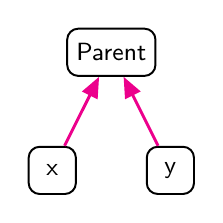
\begin{tikzpicture}[every object type/.style={shape=circle},
    edge from parent/.style=subtype]
    \entity {Parent} 
    child {node[entity] {x}}
    child {node[entity] {y}};
  \end{tikzpicture}
  \caption{Specialisatie}
  \label{fig:specialisatie}
\end{figure}


\subsubsection{T4}
\[
  x \operatorname{Gen} y \wedge y \sim z \vdash x \sim z
\] waar $x \operatorname{Gen} y$ betekent ``$x$ is een generalisatie van $y$''.

Op dezelfde manier als bij T3 (\ref{s2e:t3}), komen elementen van
generalisaties voor in het gegeneraliseerde type. Typen die gerelateerd zijn aan 
een bepaald type, zijn dus ook gerelateerd aan de generalisaties
van dat type.


\begin{figure}[b]
  \centering
  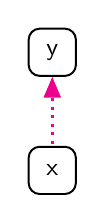
\begin{tikzpicture}[every object type/.style={shape=circle},
    edge from parent/.style={subtype,dotted}]
    \entity {y} 
      child {node[entity] {x}};
  \end{tikzpicture}
  \caption{Generalisatie}
  \label{fig:generalisatie}
\end{figure}

\subsubsection{T5}
\label{T5}
\[
  x,y \in \mathcal{G} \wedge \operatorname{Elt}(x) \sim 
  \operatorname{Elt}(y) \vdash x \sim y
\]

Als $x$ en $y$ powertypen zijn, en hun elementen typegerelateerd, 
dan zijn deze powertypen, verzamelingen van hun elementtypen,
natuurlijk ook gerelateerd.

\subsubsection{T6}
\[
  x,y \in \mathcal{S} \wedge \operatorname{Elt}(x) \sim 
  \operatorname{Elt}(y) \vdash x \sim y
\]

Zoals bij T5 (\ref{T5}), zijn als de elementen van sequentietypen 
typegerelateerd zijn, de sequentietypen zelf ook typegerelateerd.

\subsubsection{T7}
\[
  \mathcal{O}_x = \mathcal{O}_y \vdash x \sim y
\]

Als het objecttype van $x$ en die van $y$ dezelfde zijn, zijn $x$ en $y$ 
typegerelateerd.

\subsection{Voorbeeld}

Ik gebruik hier \cite[figuur 2.26]{dictaat} uit het dictaat. Ik ga de bewering 
dat alle typen behalve $C$ en $B$, $C$ en $E$, en $C$ en $F$, typegerelateerd
zijn toetsen.

\begin{align}
  A \operatorname{Gen} B               & \vdash A \sim B \\
  A \operatorname{Gen} C                & \vdash A \sim C \\
  \sqcap(D) = \sqcap(A) \wedge A \sim C & \vdash D \sim C \\
  \sqcap(D) = \sqcap(A) \wedge A \sim B & \vdash D \sim B \\
  B, E \in \mathcal{G} \wedge A \sim D  & \vdash B \sim E 
\end{align}


%
%
%
%
%
% TODO
%
%
%
%
%

\fbox{\Huge TODO}

\subsection{Conclusie}

Typegerelateerdheid is iets wat op een redelijk intu\"itief vlak werkt,
maar ook een aantal harde regels kent. Veel van die regels zijn makkelijk
beredeneerbaar, zoals bijvoorbeeld typegerelateerdheid van powertypen, en 
sommige anderen zijn iets moeilijker om te onderbouwen.

\section{Taak 3 - Constraints}

\subsection{Inleiding}

In deze taak probeer ik wat ingewikkelder contraints en restricties op
domeinmodellen te vinden, en daar wat voorbeelden bij te maken en uit te
werken. In het bijzonder ga ik het deze keer proberen op te schrijven zonder
gebruik te maken van afbeeldingen\footnote{Ik maak wel gebruik van schema's in
mijn notities, omdat het bedenken van een kloppend schema door willkeurig
opschrijven van symbolen niet echt doenbaar is.}. Ik ga ook proberen
verschillende constraints in een model te gebruiken.

\subsection{Systeem 1}
\begin{align*}
  \mathcal{P}    & = \{p1,p2,p3,p4\}\\
  \mathcal{E} & = \{A,B,C\} \\
  \mathcal{F} & = \{f,g\}   \\
  \mathcal{G} & = \emptyset        \\  
  \mathcal{S} & = \emptyset        \\
  \Spec       &\Rightarrow B \Spec A       \\
  f           & = \{p1,p2\} \\   
  g           & = \{p3,p4\} \\
  \Base (p1)   & = A         \\
  \Base (p2)   & = B         \\
  \Base (p3)   & = A         \\
  \Base (p4)   & = C        \\ 
  \total (\tau) &\text{ where } \tau = \{p1\} \\
  \total (\tau) &\text{ where } \tau = \{p2\} \\
\end{align*}


\begin{thebibliography}{9}
  \bibitem{dictaat}
    Advanced Information Models, 
    Arthur ten Hofstede en Patrick van Bommel,
    Radboud Universiteit Nijmegen,
    September 2011,
\end{thebibliography}

\end{document}
